% ---------------------------------------------------------------------------
% Project 1 slides, NLP course. DistilBERT vs BERT for text classification.
% Theme: slate-blocks (Slate_Blocks___a_Beamer_theme_with_seven_named_blocks/).
%
% Build:  tectonic -X compile main.tex     (tectonic reruns until stable)
%
% Same rule as the report: figures and tables are read from
% ../../results/figures/, where `python -m src.plots` writes them, so no
% number on a slide was typed by hand except in the prose.
% ---------------------------------------------------------------------------
\documentclass[xcolor={dvipsnames,table}, aspectratio=1610]{beamer}

\usetheme{Madrid}
\useoutertheme{miniframes}
\useinnertheme{circles}

\usepackage[T1]{fontenc}
\usepackage{amsmath}
\usepackage{booktabs}
\usepackage{adjustbox}

% The theme lives in its own folder; style.tex and its figures are found
% through the input and graphics paths instead of being copied here.
\makeatletter
\def\input@path{{Slate_Blocks___a_Beamer_theme_with_seven_named_blocks/}}
\makeatother
\graphicspath{{Slate_Blocks___a_Beamer_theme_with_seven_named_blocks/}{../../results/figures/}}

% =============================================================================
% style.tex — the palette, the named blocks, and the title page.
%
% Extracted from a course presentation given in 2025. Everything here is the
% author's own; the beamer themes underneath (Madrid, miniframes, circles) ship
% with beamer itself, so there is no third-party licence to carry.
%
% Load after \documentclass and the \usetheme lines. See README.md.
% =============================================================================

\usepackage{xcolor}
\usepackage{etoolbox}   % \BeforeBeginEnvironment, used by the block factory
\usepackage{tikz}
\usetikzlibrary{positioning}
\usepackage{makecell}   % multi-line table cells
\usepackage[most]{tcolorbox}   % the SWOT grid at the foot of this file

% -----------------------------------------------------------------------------
% THE PALETTE
%
% One colour is chosen; the rest are derived from it by colour-wheel relations,
% so the whole deck re-tints from a single line.
%
%   #bec2cb is a desaturated blue-grey. It is light, which is the point: at
%   full strength it is a background, and at !250 — beamer's syntax for a tint
%   past 100%, i.e. a darkening — it becomes the body text colour. One value
%   doing both ends of the range is what keeps the deck quiet.
%
%   Analogous          neighbours on the wheel. Closest to the theme colour,
%                      so they read as variations rather than contrasts.
%   Tetradic           two complementary pairs. Furthest apart, so these carry
%                      the blocks that must not be confused with each other.
%   Split-complementary  either side of the true complement. A softer contrast
%                      than the complement itself, which at this saturation
%                      would look like a mistake.
%
% All seven sit at the same lightness and saturation. That is deliberate: the
% hue distinguishes them, nothing else, so no block shouts louder than another.
% -----------------------------------------------------------------------------
\definecolor{ThemeColor}{RGB}{190, 194, 203}              % #bec2cb

\definecolor{AnalogousColor-1}{RGB}{193, 190, 203}        % #c1becb
\definecolor{AnalogousColor-2}{RGB}{190, 201, 203}        % #bec9cb

\definecolor{TetradicColor-1}{RGB}{203, 190, 194}         % #cbbec2
\definecolor{TetradicColor-2}{RGB}{203, 199, 190}         % #cbc7be
\definecolor{TetradicColor-3}{RGB}{190, 203, 199}         % #becbc7

\definecolor{SplitComplementaryColor-1}{RGB}{203, 193, 190} % #cbc1be
\definecolor{SplitComplementaryColor-2}{RGB}{201, 203, 190} % #c9cbbe

\setbeamercolor{normal text}{fg=ThemeColor!250}

\setbeamercolor{palette primary}   {bg=ThemeColor,           fg=ThemeColor!12.5!white}
\setbeamercolor{palette secondary} {bg=ThemeColor!87.5!white, fg=ThemeColor!12.5!white}
\setbeamercolor{palette tertiary}  {bg=ThemeColor!75!white,   fg=ThemeColor!12.5!white}
\setbeamercolor{palette quaternary}{bg=ThemeColor!62.5!white, fg=ThemeColor!12.5!white}
\setbeamercolor{structure}    {fg=AnalogousColor-1}
\setbeamercolor{section in toc}{fg=AnalogousColor-1!150}

\setbeamersize{text margin left=10mm, text margin right=10mm}
\setbeamertemplate{navigation symbols}{}

% -----------------------------------------------------------------------------
% NAMED BLOCKS
%
% Beamer gives you three: block, example, alert. This deck wanted seven, each
% naming what it holds — an example, a comment, a proposal, a reminder — and
% each in its own hue.
%
% \newcolouredblock{Environment}{Printed label}{colour} builds one. It uses
% \newtheorem for the numbering and label, and swaps the block colours around
% the environment, because beamer has no per-block colour and \setbeamercolor
% inside a frame leaks into whatever follows.
%
% The original wrote those eight lines out once per block, seven times over.
% The colours are the design; the repetition was not.
% -----------------------------------------------------------------------------
\newcommand{\blockcolours}[1]{%
  \setbeamercolor{block title}{use=example text, fg=white, bg=#1}%
  \setbeamercolor{block body} {parent=normal text, use=block title example,
                               bg=#1!25}%
}
\newcommand{\blockcoloursreset}{%
  \setbeamercolor{block title}{use=structure, fg=white, bg=structure.fg!75!white}%
  \setbeamercolor{block body} {parent=normal text, use=block title,
                               bg=block title.bg!10!bg}%
}

\newcommand{\newcolouredblock}[3]{%
  \newtheorem{#1}{\textsc{#2}}%
  \BeforeBeginEnvironment{#1}{\blockcolours{#3}}%
  \AfterEndEnvironment{#1}{\blockcoloursreset}%
}

% The seven. Rename them into your own language — the label is the second
% argument and nothing else depends on it.
%
% The environment names carry a suffix. \Example, \Definition and friends are
% already taken: amsmath and beamer's own theorem set define several of them,
% and \newtheorem fails on a name that exists. A suffix is uglier than the bare
% word and cheaper than finding out which words are free in every package a
% future deck might load.
\newcolouredblock{ExampleBox}   {Example}    {ThemeColor}
\newcolouredblock{CommentBox}   {Comment}    {AnalogousColor-1}
\newcolouredblock{ProposalBox}  {Proposal}   {AnalogousColor-2}
\newcolouredblock{ReminderBox}  {Reminder}   {TetradicColor-1}
\newcolouredblock{ProblemBox}   {Problem}    {TetradicColor-2}
\newcolouredblock{ChallengeBox} {Challenge}  {TetradicColor-3}
\newcolouredblock{DefinitionBox}{Definition} {SplitComplementaryColor-1}

% -----------------------------------------------------------------------------
% COVERING THE PAGE WITH A PHOTOGRAPH
%
% \slatecover{file} scales an image to cover the whole slide, whatever its
% aspect ratio, without distorting it. Place the result at the page centre and
% whichever dimension overruns is cropped evenly by the page edge.
%
% \includegraphics[width=\paperwidth] alone does NOT do this. The deck is 16:10
% and most photographs are 16:9; scaled to the paper's width, a 16:9 image
% comes up about a tenth of the page short and leaves a white band across the
% top. Giving both width and height distorts the picture, and adding
% keepaspectratio letterboxes it — the same gap, politely.
%
% So: measure it at full width, and if that is not tall enough, scale by height
% instead.
% -----------------------------------------------------------------------------
\makeatletter
\newsavebox{\slate@coverbox}
\newcommand{\slatecover}[1]{%
  \sbox{\slate@coverbox}{\includegraphics[width=\paperwidth]{#1}}%
  \ifdim\ht\slate@coverbox<\paperheight
    \includegraphics[height=\paperheight]{#1}%
  \else
    \usebox{\slate@coverbox}%
  \fi
}
\makeatother

% -----------------------------------------------------------------------------
% THE WATERMARK
%
% The cover photograph again, on every slide, at 6.7% — far enough down that it
% reads as paper texture rather than as an image. Anything stronger and the
% body text has to fight it.
%
% Comment this out and the deck still works; it is the one part of the design
% that costs nothing to lose.
% -----------------------------------------------------------------------------
\newcommand{\slateWatermark}[1]{%
  \usebackgroundtemplate{%
    \tikz[remember picture, overlay]{%
      \node[opacity=0.067, inner sep=0]
        at (current page.center)
        {\slatecover{#1}};%
    }%
  }%
}

% -----------------------------------------------------------------------------
% THE TITLE PAGE
%
% \slatetitlepage — a full-bleed photograph with the title in a double-stroked
% box over it, the box shaded from one analogous colour to the other.
%
% Set the five commands below it first. They are separate commands rather than
% arguments because the title page is the one place a deck wants long strings
% with markup in them, and five arguments to one command is unreadable.
% -----------------------------------------------------------------------------
\newcommand{\slateBackground}{figures/background.png}
\newcommand{\slateTitle}    {\large\textbf{\textrm{Title}}}
\newcommand{\slateSubTitle} {\small\textrm{Subtitle}}
\newcommand{\slateAuthor}   {Author}
\newcommand{\slateAffiliate}{Affiliation}
\newcommand{\slateDate}     {\today}
\newcommand{\slateLogo}     {
\includegraphics[width=0.25\paperwidth]{figures/logo.png}}

\newcommand{\slatetitlepage}{%
  \begin{tikzpicture}[remember picture, overlay]

    % opacity=0.55 — the photograph held back far enough that the title box
    % reads as something laid over it rather than as another thing at the same
    % weight. The sky keeps its blue and the maple its red down to about here;
    % below 0.5 the picture stops looking held back and starts looking faded.
    %
    % The usual recipe for this is two layers — the image at 0.65 and a white
    % rectangle at 0.15 over it. Do not bother. The page behind is white, so
    % the veil does nothing the opacity cannot: the two render to within one
    % part in 255 of a single opacity of 0.5525, which was measured, not
    % assumed. One number, one place to change it.
    \node[inner sep=0pt, opacity=0.55] at (current page.center)
      {\slatecover{\slateBackground}};

    % The double stroke and the shading are what lift the box off a photograph
    % busy enough to swallow a plain panel. shading angle=60 runs the gradient
    % across the diagonal rather than flat, so neither edge matches the photo
    % behind it for long.
    \node[
      above=0.5cm, align=center,
      draw=AnalogousColor-1!50,
      left color=AnalogousColor-1!75, right color=AnalogousColor-1!25,
      shading angle=60,
      double, double distance=0.1cm,
      inner xsep=15pt, inner ysep=10pt,
      minimum width=0.7\textwidth, text width=0.6\textwidth,
      color=AnalogousColor-2!250,
    ] (title) at (current page.center)
      {\LARGE\slateTitle \\[5pt] \small\slateSubTitle};

    \node[below=0.5cm]  (author)    at (title.south)
      {\color{AnalogousColor-1!250}\slateAuthor};
    \node[below=0.25cm] (affiliate) at (author.south)
      {\color{AnalogousColor-1!250}\small\slateAffiliate};
    \node[below=0.25cm] (date)      at (affiliate.south)
      {\color{AnalogousColor-1!250}\large\slateDate};
    \node[opacity=0.67, below=1cm]  at (affiliate.south) {\slateLogo};

  \end{tikzpicture}%
}


% ---- the palette this template mixes from ----------------------------------
%
% The helpful/harmful pair is taken from the two TETRADIC colours, which are
% the furthest apart on the wheel this palette has: greenish against pinkish,
% which is the one contrast a reader will read as good against bad without
% being told. The analogous colours are too close to the theme colour to do
% this job — at this saturation #bec9cb and #bec2cb are the same colour, and
% the two axis headers came out indistinguishable.
%
% Internal/external is the weaker distinction and gets the weaker contrast,
% at a third strength so the row bands stay under the quadrants.
\colorlet{swotHelpful} {TetradicColor-3!67}
\colorlet{swotHarmful} {TetradicColor-1!67}
\colorlet{swotInternal}{ThemeColor!33}
\colorlet{swotExternal}{TetradicColor-2!33}
\colorlet{swotInk}{AnalogousColor-1!250}
\colorlet{S}{swotHelpful!50!swotInternal}
\colorlet{W}{swotHarmful!50!swotInternal}
\colorlet{O}{swotHelpful!50!swotExternal}
\colorlet{T}{swotHarmful!50!swotExternal}

\tcbset{
  swotbox/.style     ={size=normal, boxrule=0pt, colback=#1,
                       watermark text=#1, width=.5\linewidth-5mm},
  swotheader/.style  ={size=small, boxrule=0pt, width=.5\linewidth-5mm,
                       colback=#1, valign=center, halign=center},
  swotfirstcol/.style={swotheader=#1, width=1cm},
}
% -----------------------------------------------------------------------------
% SWOT
%
% \swot{strengths}{weaknesses}{opportunities}{threats} — a 3x3 raster: a blank
% corner, two column headers, and two rows each opening with a rotated label.
%
% The four quadrant colours are MIXED rather than picked, which is what keeps
% the grid readable: every quadrant is half "helpful/harmful" and half
% "internal/external", so the two axes are legible in the colour itself and a
% reader can place a quadrant without reading its label.
%
% The letter watermarked in each quadrant is the tcolorbox colour name. That is
% deliberate — it labels the quadrant without spending a line on a heading.
% -----------------------------------------------------------------------------
\newcommand{\swotAxisHelpful}{Helpful\par\tiny (to achieve the objective)}
\newcommand{\swotAxisHarmful}{Harmful\par\tiny (to achieve the objective)}
\newcommand{\swotAxisInternal}{Internal origin\\\tiny (attributes of the thing itself)}
\newcommand{\swotAxisExternal}{External origin\\\tiny (attributes of its environment)}

\newcommand{\swot}[4]{%
  \begin{center}
  \begin{tcbitemize}[raster columns=3, raster rows=3, enhanced, sharp corners,
                     raster equal height=rows, raster force size=false,
                     raster column skip=0pt, raster row skip=0pt]
    \tcbitem[blankest, width=1cm]
    \tcbitem[swotheader=swotHelpful] {\color{swotInk}\swotAxisHelpful}
    \tcbitem[swotheader=swotHarmful] {\color{swotInk}\swotAxisHarmful}

    \tcbitem[swotfirstcol=swotInternal]
      {\rotatebox[origin=c]{90}{\parbox[t]{2.4cm}{\centering
        \color{swotInk}\swotAxisInternal\par}}}
    \tcbitem[swotbox=S] #1
    \tcbitem[swotbox=W] #2

    \tcbitem[swotfirstcol=swotExternal]
      {\rotatebox[origin=c]{90}{\parbox[b]{2.4cm}{\centering
        \color{swotInk}\swotAxisExternal\par}}}
    \tcbitem[swotbox=O] #3
    \tcbitem[swotbox=T] #4
  \end{tcbitemize}
  \end{center}%
}


% Colours the generated tabulars expect (same as docs/informe/main.tex).
\definecolor{cabecera}{HTML}{DCDCEF}
\definecolor{lila}{HTML}{E6E1F5}

\newcommand{\tabla}[1]{\begin{adjustbox}{max width=\linewidth}%
  \input{../../results/figures/#1.tex}%
\end{adjustbox}}

\slateWatermark{figures/background.png}

\renewcommand{\slateTitle}    {\large\textbf{\textrm{How Much of BERT Does Text Classification Need?}}}
\renewcommand{\slateSubTitle} {\small\textrm{A controlled comparison with DistilBERT}}
\renewcommand{\slateAuthor}   {Jose Huamani, Renzo Felix, Diego Quispe}
\renewcommand{\slateAffiliate}{Universidad de Ingenier\'ia y Tecnolog\'ia (UTEC), Lima, Peru}
% The template's logo is a placeholder; no institutional mark ships here.
\renewcommand{\slateLogo}{}

\title[BERT vs DistilBERT]{How Much of BERT Does Text Classification Need?}
\subtitle{A controlled comparison with DistilBERT}
\author[Huamani, Felix, Quispe]{Jose Huamani, Renzo Felix, Diego Quispe}
\institute[UTEC]{UTEC}
\date{NLP 2026}

\begin{document}

\begin{frame}[plain]
  \slatetitlepage
\end{frame}

% ===========================================================================
\section{\textsc{Setup}}

\begin{frame}{\textsc{The question and the setup}}

  \begin{ProblemBox}
    \small DistilBERT claims 97\% of BERT's GLUE score with half the layers.
    We tested that on three datasets.
  \end{ProblemBox}

  \vspace{1mm}
  \begin{center}\scriptsize
  \begin{tabular}{ll}
    \toprule
    \textbf{Models} & \texttt{bert-base-uncased} (12 layers, 109.5\,M) and
      \texttt{distilbert-base-uncased} (6 layers, 67.0\,M) \\
    \textbf{Data} & SST-2 (872 test sentences), AG News (7{,}600), Yelp
      Polarity (38{,}000, train cut to 100\,k) \\
    \textbf{Recipe} & AdamW at $2\times10^{-5}$, 10\% warm-up, 2 epochs, batch
      32, fp16, seed 42 \\
    \textbf{Selection} & best validation macro-F1, then one pass over test \\
    \textbf{Runs} & 24 fine-tunings plus a latency benchmark, all on one RTX A6000 \\
    \bottomrule
  \end{tabular}
  \end{center}

  \begin{ReminderBox}
    \small Only the model changes between two columns of any table. Training
    loop, splits, seed and GPU stay the same for both.
  \end{ReminderBox}

\end{frame}

% ===========================================================================
\section{\textsc{Performance}}

\begin{frame}{\textsc{Base runs}}

  \tabla{tabla_resultados}

  \vspace{2mm}
  \begin{columns}[T]
    \begin{column}{0.48\linewidth}
      \begin{ExampleBox}
        \scriptsize BERT leads SST-2 by 1.04 points and Yelp by 0.46. On AG
        News DistilBERT is ahead by 0.09, which is seven test items out of
        7{,}600. We call that a tie.
      \end{ExampleBox}
    \end{column}
    \begin{column}{0.48\linewidth}
      \begin{ReminderBox}
        \scriptsize DistilBERT scores 91.28\% on SST-2. Sanh et al.\ report
        91.3, so our splits and recipe reproduce the published number.
      \end{ReminderBox}
    \end{column}
  \end{columns}

\end{frame}

\begin{frame}{\textsc{Size, accuracy and latency}}

  \begin{columns}[c]
    \begin{column}{0.55\linewidth}
      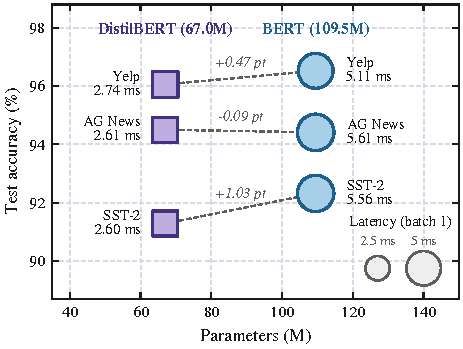
\includegraphics[width=\linewidth]{burbujas_params_acc.pdf}
    \end{column}
    \begin{column}{0.42\linewidth}
      \small DistilBERT sits 42.5\,M parameters to the left of BERT, with
      bubbles half the size. The vertical distance inside each pair is what
      the smaller model costs in accuracy.

      \vspace{3mm}
      \begin{ExampleBox}
        \scriptsize With 61\% of the parameters, DistilBERT keeps 98.9\% of
        BERT's accuracy on SST-2 and 99.5\% on Yelp. On AG News it keeps
        all of it.
      \end{ExampleBox}
    \end{column}
  \end{columns}

\end{frame}

% ===========================================================================
\section{\textsc{Efficiency}}

\begin{frame}{\textsc{Controlled latency benchmark}}

  \begin{center}
    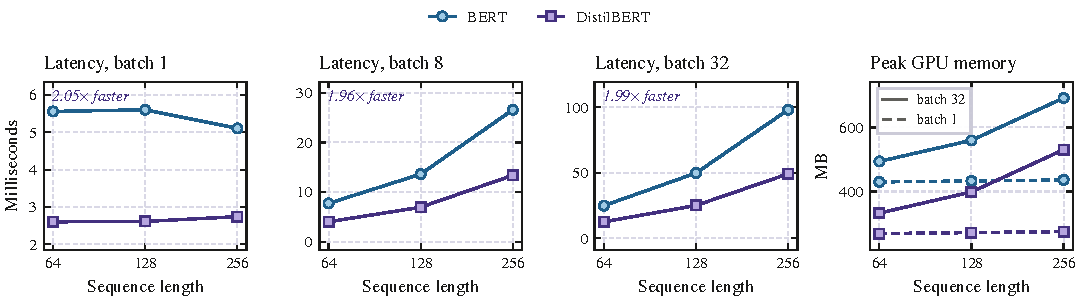
\includegraphics[width=\linewidth]{benchmark_eficiencia.pdf}
  \end{center}

  \begin{columns}[T]
    \begin{column}{0.48\linewidth}
      \begin{ExampleBox}
        \scriptsize DistilBERT wins all nine grid points, by 1.86$\times$ to
        2.15$\times$. At batch 32 and 64 tokens it handles 2{,}535 samples per
        second against 1{,}282. Its peak memory is 62\% of BERT's at batch 1
        and 77\% at batch 32 with 256 tokens.
      \end{ExampleBox}
    \end{column}
    \begin{column}{0.48\linewidth}
      \begin{ChallengeBox}
        \scriptsize The timings logged after each run put BERT ahead on SST-2
        (3.16 against 3.50\,ms). Twice the layers can't be faster. We threw
        those out and timed both models again in one process, in fp32, with
        20 warm-up passes and 50 synchronized ones.
      \end{ChallengeBox}
    \end{column}
  \end{columns}

\end{frame}

% ===========================================================================
\section{\textsc{Ablation}}

\begin{frame}{\textsc{Six classifier heads on DistilBERT}}

  \begin{columns}[T]
    \begin{column}{0.46\linewidth}
      \vspace{2mm}
      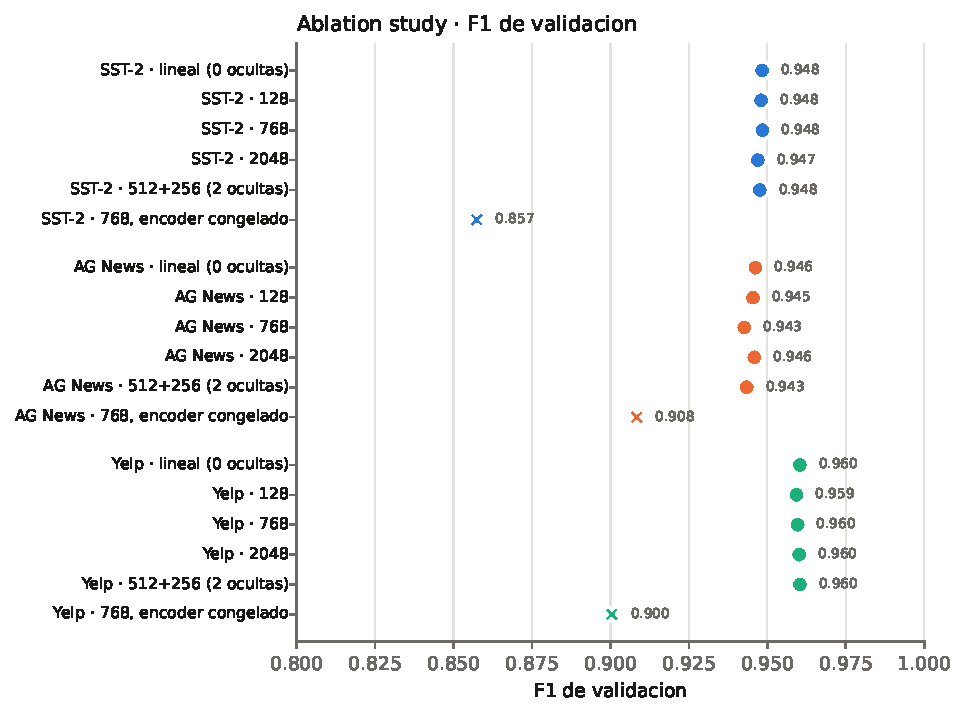
\includegraphics[width=\linewidth]{ablation.pdf}
    \end{column}
    \begin{column}{0.5\linewidth}
      \scriptsize Every head reads the \texttt{[CLS]} state. Width goes from
      128 to 2048, depth from zero to two hidden layers, and one run freezes
      the encoder.

      \vspace{2mm}
      \begin{ExampleBox}
        \scriptsize With a trainable encoder the five heads land between 95.03
        and 95.16 mean validation F1. Their order changes from dataset to
        dataset.
      \end{ExampleBox}
      \begin{ProblemBox}
        \scriptsize Freezing drops the mean to 88.87. With the same head it
        loses 9.1 points on SST-2, 5.9 on Yelp and 3.4 on AG News.
      \end{ProblemBox}
      \begin{ProposalBox}
        \scriptsize The linear head wins on the mean. It is also the smallest
        and trains fastest.
      \end{ProposalBox}
    \end{column}
  \end{columns}

\end{frame}

\begin{frame}{\textsc{The linear head on both models}}

  \tabla{tabla_mejor_config}

  \vspace{2mm}
  \begin{columns}[T]
    \begin{column}{0.48\linewidth}
      \begin{ExampleBox}
        \scriptsize BERT takes all three datasets: 1.95 points on SST-2, 0.43
        on Yelp and 0.11 on AG News.
      \end{ExampleBox}
    \end{column}
    \begin{column}{0.48\linewidth}
      \begin{CommentBox}
        \scriptsize Without its $\tanh$ pooler, BERT climbs to 92.89 on SST-2
        from 92.32. DistilBERT slips from 91.28 to 90.94, so the gap opens
        from both ends.
      \end{CommentBox}
    \end{column}
  \end{columns}

\end{frame}

% ===========================================================================
\section{\textsc{Takeaways}}

\begin{frame}{\textsc{Why the numbers look like this}}

  \begin{columns}[T]
    \begin{column}{0.48\linewidth}
      \begin{DefinitionBox}
        \scriptsize\textbf{Task.} AG News labels hang on words like
        \emph{earnings} or \emph{playoffs}, and six layers already see them.
        Both models trip on the same stories. BERT sends 140 Business items to
        Sci/Tech and 90 back, DistilBERT 140 and 92. SST-2 sentences turn on
        negation and contrast, where depth pays.
      \end{DefinitionBox}
      \begin{DefinitionBox}
        \scriptsize\textbf{Head.} Fine-tuning bends the \texttt{[CLS]} vector
        until one linear layer separates the classes.
      \end{DefinitionBox}
    \end{column}
    \begin{column}{0.48\linewidth}
      \begin{DefinitionBox}
        \scriptsize\textbf{Latency.} At batch 1, BERT barely moves with length
        (5.56, 5.61 and 5.11\,ms). The GPU waits on kernel launches, and
        DistilBERT has half as many. From batch 8 up, time grows with input
        length and DistilBERT does half the arithmetic.
      \end{DefinitionBox}
      \begin{CommentBox}
        \scriptsize Memory closes in as the batch grows. Activations add about
        the same amount to both models.
      \end{CommentBox}
    \end{column}
  \end{columns}

\end{frame}

\begin{frame}{\textsc{Conclusion}}

  \begin{itemize}\small
    \item DistilBERT is our default for these tasks. It keeps 98.9\% to 100\%
      of BERT's accuracy with 61\% of the parameters, two thirds of the memory
      and half the latency.
    \item BERT's margin has a price. On AG News, 0.11 points will rarely
      justify doubling the inference bill. On SST-2, 1.95 might.
    \item One linear layer on \texttt{[CLS]} is enough. Freezing the encoder
      is the choice that hurts.
  \end{itemize}

  \vspace{3mm}
  \begin{ProblemBox}
    \scriptsize\textbf{Limitations.} Every run used seed 42, so we have no
    intervals and gaps of a few tenths count as ties. SST-2 has 872 test
    sentences, and 1.04 points is nine of them. Two epochs is the low end of
    what BERT's authors recommend.
  \end{ProblemBox}

\end{frame}

\begin{frame}[plain]
  \centering\vfill
  {\Huge\textsc{Thank you}}\\[6mm]
  {\large Questions?}
  \vfill
\end{frame}

\end{document}
